\newcommand{\pdftitel}{Wissensbasierte Systeme - Programmentwurf}
\newcommand{\autorA}{Nico-Alexei Hein}
\newcommand{\autorB}{Andreas Rau}
\newcommand{\arbeit}{Programmentwurf}

%----------------------------------------------------------------------------
% PREFERENCES
%----------------------------------------------------------------------------
\documentclass[
	12pt,
	a4paper,
	titlepage,
	oneside
]{article}			

%Seitengroesse
\usepackage[top=1in, bottom=1in, left=1in, right=1in]{geometry}
%\usepackage{fullpage}

%Exkurse
\usepackage{blindtext}

%Zeilenumbruch und mehr geht nur am MAC!!
\usepackage[activate]{microtype} 
\usepackage{lmodern}

% Zeichencodierung
\usepackage[utf8]{inputenc}
\usepackage[T1]{fontenc}

% Zeilenabstand
\usepackage[doublespacing]{setspace}

% Index-Erstellung
\usepackage{makeidx}

% Lokalisierung (englische Sprache)
\usepackage[american]{babel}

% Anführungszeichen 
%\usepackage[babel,german=quotes]{csquotes}
\usepackage{csquotes}

%tableen
\usepackage{tabularx}

% Spezielle Tabellenform fuer Deckblatt
\usepackage{longtable}
\setlength{\tabcolsep}{10pt} %Abstand zwischen Spalten
\renewcommand{\arraystretch}{1.5} %Zeilenabstand


%Matrix
\usepackage{multirow}


% Grafiken
\usepackage{graphicx}

% Mathematische Textsaetze
\usepackage{amsmath}
\usepackage{amssymb}

% Pakete um Textteile drehen zu können, oder eine Seite Querformat anzeigen kann.
%\usepackage{rotating}
%\usepackage{lscape}

% Farben
\usepackage{color}
\definecolor{LinkColor}{rgb}{0,0,0}
\definecolor{ListingBackground}{rgb}{0.92,0.92,0.92}
\definecolor{grey}{rgb}{.3,.3,.3}


% PDF Einstellungen
\usepackage[
	pdftitle={\pdftitel},
	pdfauthor={\autor},
	pdfsubject={\arbeit},
	pdfcreator={pdflatex, LaTeX with KOMA-Script},
	pdfpagemode=UseOutlines, 			% Beim Oeffnen Inhaltsverzeichnis anzeigen
	pdfdisplaydoctitle=true, 			% Dokumenttitel statt Dateiname anzeigen.
	pdflang=eng, 						% Sprache des Dokuments.
]{hyperref}

% (Farb-)einstellungen für die Links im PDF
\hypersetup{
	colorlinks=true, 					% Aktivieren von farbigen Links im Dokument
	linkcolor=LinkColor, 				% Farbe festlegen
	citecolor=LinkColor,
	filecolor=LinkColor,
	menucolor=LinkColor,
	urlcolor=LinkColor,
	bookmarksnumbered=true 				% Überschriftsnummerierung im PDF Inhalt anzeigen.
}

\usepackage{multicol}

% Hurenkinder und Schusterjungen verhindern
% http://projekte.dante.de/DanteFAQ/Silbentrennung
\clubpenalty=10000
\widowpenalty=10000
\displaywidowpenalty=10000


\usepackage{todonotes}					% for todos

% Quellcode
\usepackage{listings}
\lstloadlanguages{Java}
\lstset{
	language=PHP,            		% Sprache des Quellcodes
	numbers=left,           		% Zeilennummern links
	stepnumber=1,            		% Jede Zeile nummerieren.
	numbersep=5pt,           		% 5pt Abstand zum Quellcode
	numberstyle=\tiny,       		% Zeichengrösse 'tiny' für die Nummern.
	breaklines=true,         		% Zeilen umbrechen wenn notwendig.
	breakautoindent=true,    		% Nach dem Zeilenumbruch Zeile einrücken.
	postbreak=\space,        		% Bei Leerzeichen umbrechen.
	tabsize=2,               		% Tabulatorgrösse 2
	basicstyle=\ttfamily\footnotesize, % Nichtproportionale Schrift, klein für den Quellcode
	showspaces=false,        		% Leerzeichen nicht anzeigen.
	showstringspaces=false,  		% Leerzeichen auch in Strings ('') nicht anzeigen.
	extendedchars=true,      		% Alle Zeichen vom Latin1 Zeichensatz anzeigen.
	captionpos=b,            		% sets the caption-position to bottom
	backgroundcolor=\color{ListingBackground} % Hintergrundfarbe des Quellcodes setzen.
}

% Glossar
\usepackage[
	nonumberlist, 					%keine Seitenzahlen anzeigen
	acronym,    	  			 	%ein Abkürzungsverzeichnis erstellen
	section,     					%im Inhaltsverzeichnis auf section-Ebene erscheinen
	toc,          					%Einträge im Inhaltsverzeichnis
]{glossaries}

%bibliographie
%\usepackage[authoryear]{natbib}
%\usepackage{apacite}

\usepackage[backend=biber,date=short,maxcitenames=2,style=apa]{biblatex}
\DeclareLanguageMapping{american}{american-apa}

\addbibresource{literature.bib}


% Fussnoten
\usepackage[perpage, hang, multiple, stable]{footmisc}

% Titel, Autor und Datum
\title{\titel}
\author{\autorA}
\author{\autorB}
\date{\datum}



% Kopf und fußzeile
\usepackage{fancyhdr} 





% Ab jetzt können auch Umlaute verwendet werden
\newcommand{\titel}{Wissensbasierte Systeme\\ Probabilistische Netze}
\newcommand{\matrikelnrA}{7146604}
\newcommand{\matrikelnrB}{4186494}
\newcommand{\kurs}{TINF12A}
\newcommand{\datumAbgabe}{Januar 2015}
\newcommand{\firmaA}{Hewlett Packard}
\newcommand{\firmenortA}{Bad Homburg}
\newcommand{\firmaB}{IBM}
\newcommand{\firmenortB}{Böblingen}
\newcommand{\abgabeort}{Stuttgart}
\newcommand{\studiengang}{Angewandte Informatik}
\newcommand{\dhbw}{Stuttgart}
\newcommand{\betreuer}{Prof. Dr. Dirk Reichardt}

\makeglossaries
%
% vorher in Konsole folgendes aufrufen: 
% makeglossaries makeglossaries dokumentation.acn && makeglossaries dokumentation.glo
%

%
% Abkürzungen --> referenz, name, beschreibung
% Aufruf mit \gls{...} oder Kurzform mit \acrshort{...}
%

\newacronym{DSRC}{DSRC}{Dedicated Short Range Communications}
\newacronym{GPS}{GPS}{Global Positioning System}
\newacronym{GUI}{GUI}{Graphical User Interface}
\newacronym{IPS}{IPS}{Indoor Positioning System}
\newacronym{INS}{INS}{Indoor Navigation System}

% Glossareintraege --> referenz, name, beschreibung
% Aufruf mit \gls{...}
%
%\newglossaryentry{Glossary-entry}{name={Glossary-entry},plural={Glossary-entries},description={A Glossary describes different things in short words.}}




\newglossaryentry{Smart_City}{name={Smart City}, description={A Smart City is a settlement area where sustainable products, services, technologies, processes and infrastructures are developed with ecologic, social and economic aspects using highly integrated information and communication technologies. }}



\clearpage

\begin{document}
	% Deckblatt
	\begin{spacing}{1}
		\begin{titlepage}
	\begin{center}
		
\includegraphics[height=2.6cm]{images/dhbw.png}
	\end{center}
	\enlargethispage{20mm}
	\begin{center}
	  \begin{spacing}{2}
	  \vspace*{9mm}	{\Large\bf \titel }\\
	  \end{spacing}
	  \vspace*{8mm}	{\large\bf \arbeit}\\

	  \vspace*{17mm}	at Course of Studies \studiengang\\
	  \vspace*{3mm} 	at the Cooperative State University \dhbw\\
	  \vspace*{12mm}	by\\
	  \vspace*{3mm} 	{\large\bf \autor}\\
	  \vspace*{12mm}	\datumAbgabe\\
	\end{center}
	\vfill
	\begin{spacing}{1.2}
	\begin{tabbing}
		mmmmmmmmmmmmmmmmmmmmmmmmmm     \= \kill
		\textbf{Supervisor}              \>  \betreuer\\
		\\
		\textbf{\autor}\\
		Student ID, Course  \>  \matrikelnr, \kurs\\
		Company      \>  \firma, \firmenort\\
		
		
	\end{tabbing}
	\end{spacing}
\end{titlepage}

	\end{spacing}
	\clearpage
	
		
	\renewcommand{\thepage}{\Roman{page}}
	\setcounter{page}{1}
	\pagestyle{plain}

	% Inhaltsverzeichnis
	\begin{spacing}{1.1}
		\setcounter{tocdepth}{3}
		\tableofcontents
	\end{spacing}
	\clearpage
	
	% Abbildungsverzeichnis
	%\cleardoublepage
	%\phantomsection \label{listoffig}
	%\addcontentsline{toc}{section}{List of figures}
	%\listoffigures
	%\clearpage
	
	% Abkürzungsverzeichnis
	% vorher in Konsole folgendes aufrufen: 
	%	makeglossaries makeglossaries dokumentation.acn && makeglossaries dokumentation.glo
	\printglossary[type=\acronymtype]
  	\cleardoublepage	
	
	\renewcommand{\thepage}{\arabic{page}}
	\setcounter{page}{1}


	
	\pagestyle{fancy} 
		
	\rhead{} \chead{\textcolor{grey}{\thepage}} \lhead{} 
	\lfoot{\textcolor{grey}{\today}} \cfoot{} \rfoot{\textcolor{grey}{Nico-Alexei Hein, Andreas Rau}} 
		
	\renewcommand{\headrulewidth}{0.2mm} 
	\renewcommand{\footrulewidth}{0.2mm} 
	\setlength{\headheight}{0mm}
	
	
	% Inhalt
	\newpage
\section{Aufgabenstellung}
\begin{quote}
\glqq Entwickeln Sie eine Software, welche bei Eingabe (Datei, vgl. Beispielformat) von Testdaten die entsprechenden Klassifikationen mit Hilfe der Bayes Netze geeignet bestimmt und ausgibt.\grqq
\end{quote}
\textit{Wortlaut der Aufgabenstellung}
\section{Herangehensweise und Ansatz}
Mit Probabilistichen Netzen (Bayesian Networks) werden insbesondere Aussagen über unbeobachtete statistische Variablen gemacht, welche zuvor aus Beobachteten stochastisch abhängigen Variablen gefolgert wurden.

Ziel dieser Aufgabe ist eine Prognose der Hochschulqualifikation mittels probabilistischem Netz zu realisieren, bei der eine Wahrscheinlichkeitsvariable (die Hochschulqualifikation) vorhergesagt wird. Die Klassifikation der Datensätze folgt daher immer dem selben Schema. (Es eigneten sich von daher auch andere weniger flexible Algorithmen des maschinellen Lernens wie One Rule oder Entscheidungsbäume.)

Um in einem probabilistischen Netz schlussfolgern zu können, muss die Struktur des Netzes festgelegt sein (Knoten = Zufallsvariablen und gerichtete Kanten = „direkter Einfluss“) und die Parameter eines jeden Knotens (Conditional Propability Table - CPT) müssen bekannt sein. 

Das Erstellen von probabilistischen Netzten kann entweder manuell oder automatisch erfolgen. Wird ein probabilistisches Netz automatisch generiert, so kann man weiter Unterscheiden zwischen Parameterlernen und Strukturlernen. Bei erstem ist die Struktur schon vorgegeben - also oftmals manuell erstellt - und die CPT werden aus vorliegenden Datensätzen generiert. 
Beim Strukturlernen wird das gesamte Netz aus den Trainigsdaten generiert. Die manuelle Arbeit wird somit minimiert. Das manuelle Erstellen der Netze ist insbesondere dann sinnvoll, wenn die logischen Abhängigkeiten eines Netzes wie auch die Wahrscheinlichkeiten bekannt sind. Sind die Abhängigkeiten bekannt, nicht jedoch die Wahrscheinlichkeiten so eignet sich das Parameterlernen auf Testdaten. Wird es zudem kompliziert die Abhängigkeiten zwischen den Variablen zu erkennen kann das Strukturlernen abhilfe schaffen.
\clearpage
\subsection*{Analyse der gegebenen Informationen}\label{analyse}
Die 17 in dem Dokument \lstinline{P_A02.csv} gegebenen beobachteten Variablen sind:
\begin{singlespace}
\begin{multicols}{2}
\begin{enumerate}
	\item Qualifikation
	\item Schnitt
	\item Bundesland
	\item Mathe
	\item Physik
	\item Deutsch
	\item Schultyp
	\item OLT-Mathe
	\item OLT-Deutsch
	\item Studierfähigkeitstest
	\item Alter
	\item Geschlecht
	\item Jahreseinkommen der Eltern
	\item Staatsbürgerschaft
	\item Studiengang
	\item Zwischenkalk
	\item Abschluss
\end{enumerate}
\end{multicols}
\end{singlespace}

Bevor die Abhängigkeiten der Variablen und die Variablen selbst diskutiert werden, präzisieren wir an dieser Stelle die Aufgabenstellung unter Beachtung der bis hierhin gewonnenen Erkenntnisse:  


Das zu erstellende probabilistische Netz soll eine Empfehlung für den geeignetsten Studiengang ausgeben oder vom Studium abraten. Da es sich bei dem Tool um ein Online-Beratungssystem handelt welches vor Studienantritt ausgeführt wird, kann davon ausgegangen werden, dass die Variablen 15 - 17 unbekannt sind. Des weiteren sind ausschließlich die Variablen \glqq Studiengang\grqq \ und \glqq Abschluss\grqq \ für die Aussage relevant, wodurch die Variable Zwischenkalk überflüssig wird und nicht weiter betrachtet wird. 

Die Hochschulqualifikation kann durch zwei Abfragen im probabilistischen Netz erfolgen. Erstere mit $P(Abschluss|...)$ wobei aus der Prognose \glqq nicht geschafft\grqq \ das Abraten vom Studiengang folgt. Und zweite mit $P(Studiengang|...)$ welche den zu Empfehlenden Studiengang prognostiziert. 

Bei Betrachtung der Variablen fallen einige Abhängigkeiten sofort ins Auge wie \glqq Mathe\grqq \ und \glqq OLT-Mathe\grqq \ oder die allgemein Bekannte Abhängigkeit zwischen\glqq Jahreseinkommen der Eltern\grqq \ und \glqq Qualifikation\grqq. Bei vielen anderen Variablen ist es jedoch nur möglich stochastische Abhängigkeiten zu vermuten wie zwischen \glqq Qualifikation\grqq \ und \glqq Studierfähigkeitstest\grqq. Da diese Abhängigkeiten auch nur statistisch belegt werden können ist eine direkte Definition der Struktur des Netzes so nicht möglich. Eine Ausführliche Beschreibung zur Herangehensweise bei der Erstellung der Struktur folgt aus diesem Grund unter Abschnitt \ref{erstellen}. 
  
Da für die Anwendung der Bayes’schen Regel der Satz der vollständigen Ereignisdisjunktion gilt, sollten alle Wahrscheinlichkeitsvariablen diskret sein. Aus diesem Grund werden im folgenden Abschnitt alle Variablen auf ihre Eigenschaften untersucht und ggf. diskretisiert (wobei kontinuierliche Variablen auf einen qualitativen diskreten Raum abgebildet werden). Dabei wird beachtet, das der Informationsverlust der durch die Einteilung in Klassen entsteht möglichst gering bleibt. 

%Nominalskala: unterschidbar durch Bezeichnung
%Ordinalskala: vergleichbar
%Metrische Skala (Kardinalskala): messbar mit maßstab (Intervallskala wenn nullpunkt willkürlich)

\section{Diskretisierung der Wahrscheinlichkeitsvariablen}
Für die Definition der diskreten Klassen kann kein Gesetz angewandt werden. Da wir hier jedoch vor einem Problem, ähnlich dem eines Histogramms stehen, können wir uns an der in der Mathematik Vorlesung vorgestellten Faustregel (für $n<1000$) zur Bestimmung der Anzahl der Klassen $number \sim \sqrt{n}$,  wobei n die Größe der Domäne darstellt, orientieren \parencite{kloess}.

Wie im Einzelnen abgebildet wird, ist nun aufgelistet:

\paragraph{Die Qualifikation} ist gegeben durch \\
$Rg(Qualifikation)=\{Abitur, FH Reife, Meister, Techniker\}$
\paragraph{Der Schnitt} ist zwar eine diskrete Wahrscheinlichkeitsvariable, doch sie hat mit ihren Verwirklichungen $\{1.0, 1.1, … 4.0\}$ (ab 4.1 gilt als nicht bestanden) 31 Ausprägungen. Für eine bessere Vergleichbarkeit sind nicht mehr als 20 Klassen empfehlenswert \textcite{kloess}. Durch $\sqrt{31}=5.6$ kommen wir auf Intervalle von $[0,0.5]$ und 6 Klassen:
\begin{equation*}
\begin{split}
	Rg(Schnitt) = & \{x_1=[1.0,1.4], x_{1.5}=[1.5,1.9], x_2=[2.0,2.4], x_{2.5}=[2.5,2.9]\}  \\ 
				  & \cup \{x_3=[3.0,3.4], x_{3.5}=[3.5,4.0]\}
\end{split}
\end{equation*}
\paragraph{Bundesland} Auch wenn in den Testdaten nur wenige Bundesländer Auftauchen, kann das Netz mit allen möglichen Ausprägungen der Variable „Bundesland“ erstellt werden:
$Rg(Bundesland) = \{ Schleswig-Holstein, Hamburg, Bremen, \\ Mecklenburg-Vorpommern, Berlin, Brandenburg, Sachsen, \\ Sachsen-Anhalt, Niedersachsen, Thüringen, Nordrhein-Westfahlen, \\ Rheinland-Pfalz, Saarland, Hessen, Baden-Württemberg, Bayern\}$\\ Die Wahrscheinlichkeiten für in den Testdaten nicht vorkommende Bundesländer müssten mit minimalen werten definiert werden. 
\paragraph{Mathe} Der Schnitt wird um eine Klasse erweitert $Rg(Mathe) = Rg(Schnitt) \cup \{'keine'\}$. Der Wert \glqq keine\grqq \ kann beobachtet werden. Es bedeutet in diesem fall nicht, das keine Daten vorliegen, sondern, das es keine Note gibt. (Vergl. Schultyp und Studierfähigkeitstest)

\paragraph{Physik} Es gilt selbiges wie bei Mathe: $Rg(Physik) = Rg(Mathe)$
\paragraph{Deutsch} Es gilt selbiges wie bei Mathe: $Rg(Deutsch) = Rg(Mathe)$
\paragraph{Schultyp} Aus den Testdaten lassen sich vier Ausprägungen ableiten: 
\begin{equation*}
\begin{split}
Rg(Schultyp) =  & \{Allgemeines Gymnasium, Technisches \\
				& Gymnasium, Wirtschaftsgymnasium, n.a.\}
\end{split}
\end{equation*}
Es ist jedoch anzunehmen, dass bei Angabe von \glqq n.a.\grqq \ diese Variable unbeobachtet ist. Damit entfernen wir diese Ausprägung für die Variable Schultyp. 

\paragraph{OLT-Mathe} Aus den Testdaten lässt sich schließen, dass sich beim OLT 100 Punkte erzielen lassen. Durch $number \sim \sqrt{100}$ ergeben sich 10 Klassen. Außerdem scheint dieser Test pflicht zu sein. 
\begin{equation*}
\begin{split}
Rg(OLTM)= 	& \{ x_1=[0,10], x_2=[11,20], x_3=[21,30], \\
			& x_4=[31,40], x_5=[41,50], x_6=[51,60], x_7=[61,70], \\
			& x_8=[71,80], x_9=[81,90], x_{10}=[91,100]\}
\end{split}
\end{equation*}
\paragraph{OLT-Deutsch} Für OLT-Deutsch gilt selbiges wie für OLT-Mathe \\ $Rg(OLTD)=Rg(OLTM)$
\paragraph{Studierfähigkeitstest} Anhand der Testdaten für den Test lässt sich ablesen, das dieser Test keine Pflicht ist, und die Ergebnisse im Interval $[0,1000]$ liegen. Da hier keine höhere Präzision als bei den OLTs erwartet werden kann, ist eine genauere Differenzierung auch nicht notwendig. Der Wert \glqq n.a.\grqq \ bedeutet, dass hier keine Daten vorliegen. Damit wird diese Variable unbeobachtet, was uns dazu veranlasst diesen Wert zu entfernen.  Wir legen somit für die Klassen fest: 
\begin{equation*}
\begin{split}
Rg(Studienfähigkeitstest)=\{ & x_1=[0,100], x_2=[101,200], x_3=[201,300], \\
	 						 & x_4=[301,400], x_5=[401,500], x_6=[501,600], \\
							 & x_7=[601,700], x_8=[701,800], x_9=[801,900], \\ 
							 & x_{10}=[901,1000] \}
\end{split}
\end{equation*}
\paragraph{Alter} Um hier eine Abgeschlossene Menge zu bekommen, beschränken wir uns auf die in den Testdaten vorkommenden 17 - 27 Akzeptiert. Diese 11 Ausprägungen werden vorerst beibehalten. \\ $Rg(Alter)=\{[17,27]\}$ 
\paragraph{Geschlecht} Für das Geschlecht werden zwei Klassen angenommen. Ethische Fragen hierzu werden der Einfachheit halber ignoriert. $Rg(Geschlecht) = \{m,w\}$
\paragraph{Jahreseinkommen der Eltern} Bei den Jahreseinkommen lässt sich kein abschließender Rahmen finden. Aus diesem Grund nähern wir uns über des Intervall angegeben in den Testdaten ($[36k,209k]$).Über $\sqrt{174}$ erhalten wir 13 Klassen. Da jedoch 13 Klassen - für die relative Wahrscheinlichkeiten auf Basis von nur 100 Datensätzen ausgerechnet werden - sehr viel sind verwenden wir stattdessen nur 10 Klassen: 
\begin{equation*}
\begin{split}
Rg(Jahreseinkommen)= 	& \{x_1=[0,50k], x_2=[51k,60k], x_3=[61k,70k], x_4=[71k,80k], \\
						& x_5=[81k,90k], x_6=[91k,100k], x_7=[101k,110k], \\
						& x_8=[111k,120k], x_9=[121,130], x_{10}=[131,\infty]\}
\end{split}
\end{equation*}

\paragraph{Staatsbürgerschaft} Aus den Testdaten lassen sich drei Klassen ableiten: \\ 
$Rg(Staatsbürgerschaft) = \{deutsch, EU Buerger, Non European\}$
\paragraph{Studiengang} Aus den Testdaten lassen sich die folgenden fünf Studiengänge und damit Klassen ableiten: \\
\begin{equation*}
\begin{split}
	Rg(Studiengang) = 	& \{Maschinenbau, Soziale Arbeit, Elektrotechnik, \\
						& Wirtschaftswissenschaften,  Informatik\}
\end{split}
\end{equation*}
\paragraph{Zwischenkalkulation} Der Schnitt wird erweitert: 
\begin{equation*}
\begin{split}
Rg(Zwischenkalkulation) = & Rg(Schnitt) \\
							& \cup \{Abgebrochen, x_{4}=[4.1,4.4], \\
							& x_{4.5}=[4.5,4.9],  x_{5}=[5.0,5.4], x_{5.5}=[5.5,5.9]\}
\end{split}
\end{equation*}
\textit{Die 4.0 wird noch auf die $x_{3.5}$ gemapped, da diese noch als bestanden gilt.}

\paragraph{Abschluss} Es gilt selbiges wie für die Zwischenkalkulation. 

\subsection*{Umsetzung}
Die oben aufgeführten Klassen werden auf die Testdaten durch ein kleines Java Tool angewandt. Zuvor haben wir jedoch die Datei \lstinline{P_A02.csv} in UTF-8 encoded um einfacher alle Umlaute in Java erkennen zu können. (Beim Einlesen werden zudem alle Kommata gegen Punkte ersetzt um das Erkennen von Zahlen in Java leichter zu gestalten.)


\lstinputlisting{content/src/diskret.java} %Student ohne toAbgebrochen und toAlter


In dem vorausgegangenen Quelltext sehen wir die Methode \glqq transform\grqq, die \glqq n.a.\grqq \  aus den Testdaten entfernt, und durch ein Sternchen ersetzt, welches für \glqq unbeobachtet\grqq \ steht. Im Anschluss werden in der Methode die Funktionen aufgerufen, welche die Diskretisierung vornehmen. Diese sind analog zu den vorausgegangenen Angaben zu verstehen. 



\section{Aufstellen des Probabilistischen Netzes}\label{erstellen}

Nun kommen wir zurück zu der Diskussion der Abhängigkeiten. Hier betrachten wir die Variable \glqq Zwischenkalk\grqq \ nicht mehr näher, da sie weder zu den beobachteten noch zu den abgefragten Variablen gehört. 
Von den folgenden Abhängigkeiten ist sehr Wahrscheinlich auszugehen:\\
(Notation: X  \textasciitilde \ Y steht für X abhängig von Y)
\begin{itemize}
	\item OLT-Mathe \textasciitilde \ Mathe
	\item OLT-Deutsch \textasciitilde  \ Deutsch
	\item Schnitt \textasciitilde \  Mathe $\wedge$ Deutsch
	\item Qualifikation \textasciitilde \ Schultyp
\end{itemize}

\textit{Bei der Aufstellung dieser Liste haben wir uns auf die gegebenen Sachzusammenhänge und unseren Verstand verlassen.}

Bei anderen Beziehungen können begründete Vermutungen aufgestellt werden. In der folgenden Liste haben wir einige Vermutungen formuliert.

\begin{itemize}
	\item Studierfähigkeitstest \textasciitilde \ Mathe $\wedge$ Deutsch $\wedge$ Physik $\wedge$ Schnitt \textit{ - Es könnte sich jedoch auch nur um eine Teilmenge dieser handeln, oder weitere Variablen umfassen.}
	\item Abschluss \textasciitilde \ Jahreseinkommen \textit{ - Über derartige zusammenhänge wird häufig in der Politik diskutiert.}
	\item Qualifikation \textasciitilde  \ Jahreseinkommen \textit{ - Diese Aussage nimmt auch die politischen Diskussionen zum Thema als Grundlage}
	\item Studierfähigkeitstest \textasciitilde \  Qualifikation $\wedge$ Schultyp $\wedge$ Schnitt $\wedge$ Bundesland \textit{ - Diese Vermutung basiert der Annahme, das der Test nicht ganz unabhängig von anderen Leistungen und Umständen sein kann. Die gewählten Variablen könnten einem Betrachter einen groben Überblick über den bisherigen Bildungsweg verraten.}
\end{itemize}

Über weitere Abhängigkeiten lassen sich Vermutungen aufstellen, die ohne Beweis einer Abhängigkeit zu Missverständnissen oder falschen Annahmen führen können. So immer die Abhängigkeit einer Variable von der Staatsbürgerschaft oder des Geschlechts. Ebenfalls kritisch ist das Alter. 

Wegen möglichen ethischen Konflikte haben wir uns dazu entschieden die Daten für sich sprechen zu lassen und automatisiertes Strukturlernen anzuwenden. So können wir auf einzelne Tests in denen wir Abhängigkeiten prüfen verzichten. 

\subsection{Strukturlernen}
Nach vorangegangener Recherche haben wir das Tool \lstinline{org.openmarkov.jar} ausfindig gemacht, welches die Möglichkeit des strukturellen Lernens bietet. Ein Screenshot des Tools findet sich im Anhang unter \ref{org.openmarkov}. Das Strukturlernen ist über das heuristische Optimierungsverfahren des Bergsteigeralgorithmuses implementiert. 

Ein erster Durchlauf vollautomatisierten Strukturlernen resultiert in folgendem Netz:
\begin{center}
	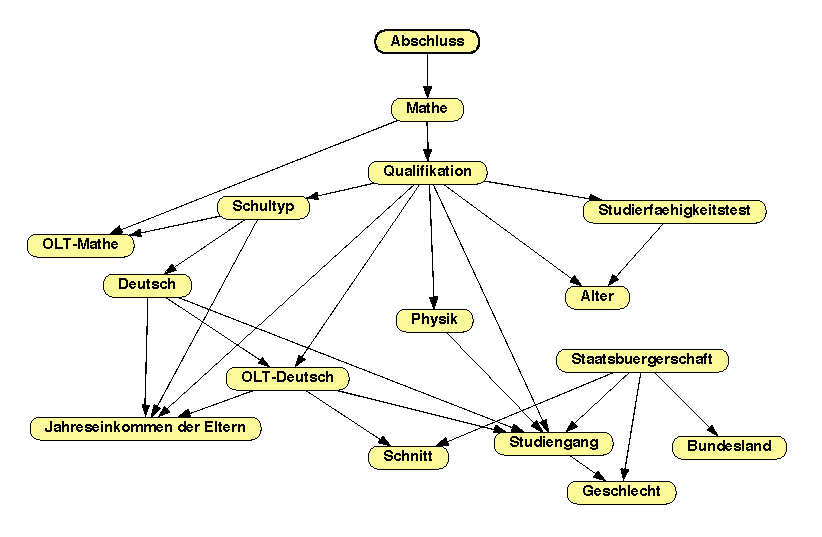
\includegraphics[width=1.00\textwidth]{content/pictures/autoNetwork.png}
\end{center}

Es kann beobachtet werden, dass bereits fast alle als sehr Wahrscheinlich angenommenen Abhängigkeiten vertreten sind. Wieder erwarten scheint der Schnitt jedoch Stärker von OLT-Deutsch und der Staatsbürgerschaft abzuhängen als von Mathe und Deutsch. Unter den weiteren vermuteten Abhängigkeiten finden sich nur sehr wenige wieder, was jedoch durchaus Plausibel ist, da es sich nur um wage Vermutungen handelte. Schauen wir jedoch genauer auf die Abhängigkeiten, so finden wir Abhängigkeiten die uns an der kompletten Korrektheit zweifeln lassen. So hängt Mathe z.B. direkt vom Abschluss ab, Deutsch jedoch vom Schultyp, der wiederum von der Qualifikation und diese von Mathe anhängt. Ein zweites Beispiel ist der Studierfähigkeitstest welcher ausschließlich von der Qualifikation abzuhängen scheint.   
Wegen dieser Zweifel starten wir einen Zweiten Anlauf, bei dem wir statt auf vollautomatisiertes lernen auf interaktives lernen setzen. 
 
\subsubsection*{Strukturlernen mit Einflussnahme}
Beim interaktiven Lernen können wir direkten Einfluss auf die zu setzenden Links nehmen. Dabei bekommen wir als User eine Liste angezeigt die uns in Frage kommende Links mit einer zugehörigen Motivation anzeigt. Es bleibt entsprechend die Möglichkeit Abhängigkeiten zu ignorieren und/oder das Netzwerk durch die Reihenfolge des Hinzufügens der Links zu beeinflussen. 

\begin{center}
	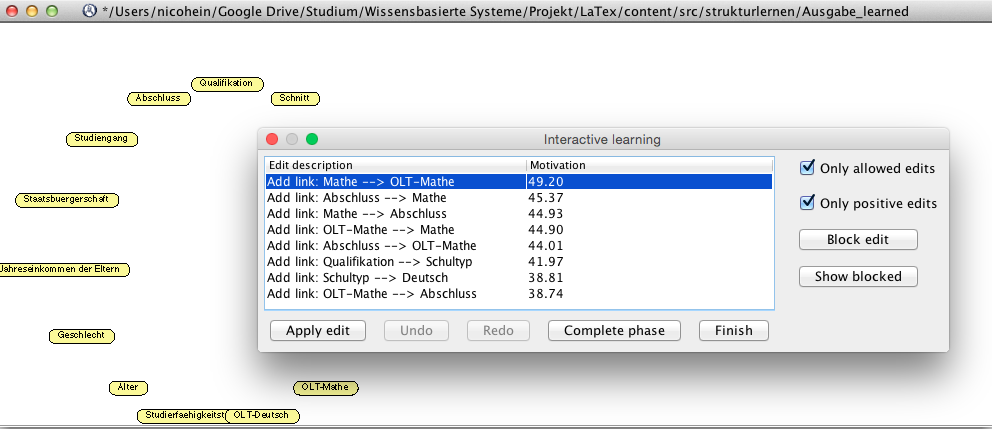
\includegraphics[width=1.00\textwidth]{content/pictures/interaktive.png}
\end{center}

Eine Liste in welcher Reihenfolge wir die Links hinzugefügt haben findet sich im Anhang unter \ref{interactive}.

Das Resultat ist folgendes:

\begin{center}
	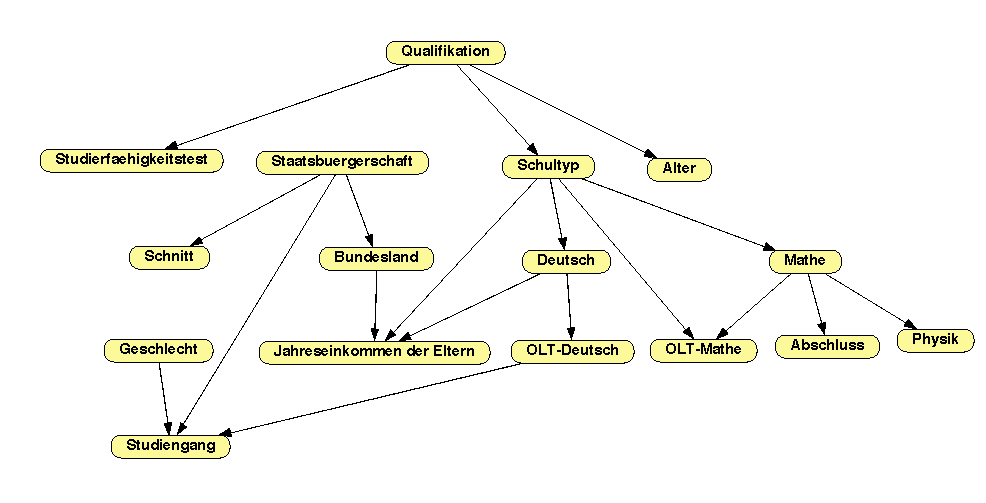
\includegraphics[width=1.00\textwidth]{content/pictures/interNetwork.png}
\end{center}

Das abgebildete Netz ist deutlich strukturierter als das welches komplett automatisch generiert wurde. Hier finden sich nun auch die Symmetrien von OLT Mathe \textasciitilde \ Mathe und OLT Deutsch  \textasciitilde \ Deutsch deutlicher wieder. Überraschend ist z.B. dass der Abschluss nur direkt von Mathe abhängt. Letztendlich finden wir auch in diesem Netz - auch wenn es plausibler erscheint - noch Zusammenhänge die nicht ganz unseren Erwartungen entsprechen. 

\textit{Die weitere Entwicklung wird jetzt am Beispiel des zweiten Netzes vorgestellt. Ein vergleich der Performance folgt dann unter \ref{test}.}

Die mithilfe von  \lstinline{org.openmarkov.jar} erstellten Netze setzten wir nun in Netica um. Netica wurde beriets in der Vorlesung ausführlich besprochen und wird aus diesem Grund hier nicht weiter Diskutiert.

\textit{\textbf{Bemerkung:} Bei der Umsetzung übernehmen wir für die Variablen alle Klassen die auch in den Testdaten vorkommen, nicht alle Möglichen.}

Der nächste Schritt zu einem voll funktionstüchtigen Netz ist das aufstellen der CPT. Diese erstellen wir durch Parameterlernen in Netica. Wir wählen diesen Weg, da die Wahrschinlichkeiten nicht gegeben sind sondern lediglich absloute Häufigkeiten, aus denen wir die relativen errechnen können. Dies kann ein Algorithmus zuverlässiger und schneller als wir es per Hand könnten. 

\subsection{Parameterlernen}
\textit{\textbf{Bemerkung: } Da Netica in der uns zur verfügung gestellten Version nur 15 Nodes unterstützt, wir ohne die Zwischenkalkulation noch immer 16 haben mussten wir uns für eine weitere Variable die wegfällt entscheiden. Da bei der interaktiven Erstellung des Netzes eine sehr hohe Abhängigkeit von Mathe und Physik festgestellt wurde (Motivation 81.03), und Physik in beiden Netzen die Erreichbarkeit von den anderen Nodes nicht beeinflusst (Qualifikation - Studiengang existiert neben Qualifikation - Physik - Studiengang (im ersten Netz) oder Mathe - Physik ist der einzige Link zu Physik (im zweiten Netz)) haben wir uns für diese Variable entschieden.}

Für das Parameterlernen erscheint es sinnvoll die Daten in Test und Trainingsdaten einzuteilen. Da wir jedoch nur einen recht kleinen Datensatz mit 100 Elementen haben ist der zu erwartende Qualitätsverlust des Gelernten bei einer Aufteilung sehr hoch. Die in der Data Mining Vorlesung  vorgestellte Holdout Methode geht mit diesem Dilemma so um, das etwa 10\% der Daten zum Testen reserviert werden, während die restlichen 90\% zum Training verwandt werden. \parencite{schmeier}). 
Da uns dann jedoch nur noch 10 Testdatensätze bleiben und auch mit stratisfaction oder der repeated-holdout Methode keine wesentliche Besserung zu erwarten ist, wählen wir den selben Datensatz zum Testen wie zum Lernen. \textit{Annahme: Dies ist bei probabilistischen Netzten nicht so kritisch wie bei 1 Rule oder Regelbäumen, da wir aus der absoluten Häufigkeit eine Relative berechnen, und keine starren Regeln definieren. Was zu dieser Überlegung veranlasst hat war der Versuch eine representative Teilmenge zu entnehmen. Dies hat sich als quasi unmöglich entpuppt, da wir es mit weit mehr als 100  ($(Mathe) 7 * (Deutsch) 7 * (OLT Mathe) 10 * ...$)  Kombinationsmöglichkeiten zu tun haben. Was bedeutet, dass jeder Datensatz schon jetzt sehr ausschlaggebend sein kann, und sich letztendlich das Netz mit jedem fehlenden Datensatz signifikant verschlechtert.} 

\textbf{Für das Parameterlernen bietet Netica u.a. die Funktion \lstinline{Cases -> Learn -> Learn using EM} an, die wir genutzt haben.}

Um diese Funktion zu Nutzen müssen die Daten als "netica case file" vorliegen. Die Bedingungen für dieses Dateivormat finden sich unter dieser URL: \url{http://www.norsys.com/WebHelp/NETICA/X_Case_File_Format.htm}. Da wir die Daten bereits eingelesen haben für die Diskretisierung muss lediglich die Ausgabe für Netica folgendermaßen angepasst angepasst werden:

\lstinputlisting{content/src/neticaout.java}

\section{Test und Anpassungen}\label{test}
Das Testen der Netze haben wir über die Netica Funktion \lstinline{Cases -> Test with Cases} durchgeführt. Dabei haben wir insbesondere die \glqq Errorrate\grqq \ im Blick. Aus den unter Abschnitt \ref{analyse} genannten Gründen testen wir auf die beiden Variablen Abschluss und Studiengang. 

%TESTS

%Interaktiv-stars						Studiengang: 41%		Abschluss:	47%		
%interaktiv-stars-abgebrochen			Studiengang: 41%		Abschluss:	8%
%interaktiv-stars-abgebrochen-alter		Studiengang: 41%		Abschluss:	8%	

%autostruktur-stars						Studiengang: 28%		Abschluss:	47%
%autostruktur-stars-abgebrochen			Studiengang: 28%		Abschluss:	8%
%autostruktur-stars-abgebrochen-alter	Studiengang: 28%		Abschluss:	8%

%TESTDATEN
%Ausgabe-stars
%Ausgabe-stars-abgebrochen
%Ausgabe-stars-abgebrochen-alter

%TEST WITH CUSTUM TEST FUNCTION

%interaktiv-stars-abgebrochen-alter				Studiengang: 17%
%autostruktur-stars-abgebrochen-alter			Studiengang: 11%



\paragraph{Erster Test: }Beim Test des interaktiv erstellten Netzes mit allen Testdaten erhalten wir eine Errorrate von 41\% für den Studiengang und eine von 47\% für den Abschluss. Beim test des automatisch generierten Netzes eine von 28\% für den studiengang und eine von 47\% für den Abschluss.

\paragraph{Interpretation des ersten Tests: } Beide Errorraten sind erstaunlich hoch, dafür das wir mit den selben Daten testen, mit denen wir auch das Netzt trainiert haben. Bei dem interaktiv erstellten Netz jedoch für den Studiengang nochmals deutlich schlechter. Für den Abschluss schenken sich die beiden Netze nichts. Betrachten wir den Abschluss genauer so fällt auf, das wir derzeit versuchen vorherzusagen ob das Studium abgebrochen wird, und wenn nicht wie es abgeschlossen wird. Zweites erschwert allerdings die Vorhersage unnötig, da es nicht von maßgeblichem Interesse ist. Deswegen korrigieren wir die Ausprägungen der Variable Abschluss auf $Rg(Abschluss) = \{Abgebrochen, Nicht Abgebrochen\}$.

\paragraph{Zweiter Test: } Mit den nun korrigierten Netzen, bei denen der Abschluss nur noch zwei Werte annehmen kann, erhalten wir jeweils die Errorrate 8\% für den Abschluss. Für den Studiengang ändert sich nichts.
 
\paragraph{Interpretation des zweiten Tests: }  Die Errorrate zur vorhersage des Abschlusses konnten wir so wesentlich verbessern. Da die Vorhersage für den Studiengang gleichbleibend schlecht ist versuchen wir über eine Korrektur der Klassen für das Alter weiter zu kommen.
Wir haben uns dazu entschieden drei Altersgruppen zu erstellen wobei wir uns an der Menge der Datensätze die in jede Klasse fallen würden orientierten:  $Rg(Alter) = \{x_{1}=[-\inf,17], x_{1}=[18,19] , x_{1}=[20,+\inf] \}$ (Mit diesen Klassen fallen 16\% der Datensätze in die erste Klasse 55\% in die Zweite und 29\% in die Dritte. 

\paragraph{Dritter Test: } Die beiden neuen Netze haben die selben Errorraten für Studiengang und Abschluss wie bei dem vorherigen Test. 

\paragraph{Interpretation des dritten Tests: } Dadurch das sich keine Änderungen mehr feststellen ließen, weder Verbesserung noch Verschlechterung, belassen wir es nun damit an den Klassen Änderungen vorzunehmen. Die neue Alterseinteilung behalten wir bei, um mit späterem Testeingaben flexibler umzugehen. 


Da in der Aufgabenstellung nicht spezifiziert wird, ob die Klassifizierung beschränkt ist auf eine Klasse oder nicht sehen wir eine Möglichkeit die Vorhersage zu verbessern, indem wir statt einem konkreten Studiengang den wir empfehlen eine Liste ausgeben in dem die Studiengänge nach ihren Ergebnissen im Netz sortiert werden. Wir sehen nun eine Vorhersage als erfolgreich an, wenn sich die tatsächliche Klasse in den ersten beiden Feldern der Liste befindet. (Zur Sortierung siehe Abfragen unter \ref{abfragen})
 
\paragraph{Vierter Test: }Um dieses neue Verständnis zu testen war eine eigene Testfunktion notwendig. In dem folgenden Code ist vor allem Zeile 17 entscheidend. (Testen wir auf einen direkten Treffer so erhalten wir die selben Resultate, wie Netica.)

\lstinputlisting{content/src/test.java}

In dem wir nun diesen Test anwenden, können wir feststellen, das die Errorrate für das automatisch erstellte Netz bei 11\% liegt, also in 89\% der fälle die Richtige Klassifikation an erster ODER zweiter Stelle der Liste ist. Für das interaktiv erstellte Netz verbessert sich Die Rate auf 17\%. 

Für die Abfragen in dem Tool verwenden wir dementsprechend das automatisch erstellte Netz und geben statt eines einzelnen Studiengangs die zwei wahrscheinlichsten Studiengänge aus. 

\section{Abfragen}\label{abfragen}
Wie bereits unter Abschnitt \ref{analyse} beschreiben kann die Hochschulqualifikation durch zwei Abfragen im probabilistischen Netz mit $P(Abschluss|...)$ und $P(Studiengang|...)$ erfolgen.\\

Im folgenden Codeabschintt ist die Abfrage von $P(Abschluss|...)$ gezeigt, mit der Annahme das alle beobachteten Variablen bereits auf das Netz angewendet wurden.

\lstinputlisting{content/src/abschluss.java}

Haben States die selbe Wahrscheinlichkeit, so wird \glqq nichtAbgebrochen\grqq \ gewählt.

Bei der Ausgabe des Studiengangs wollen wir nicht behaupten, dass es sich um einen passenden Studiengang für die jeweilige Person handelt, sondern lediglich um die zutreffendsten Studiengänge aus der Liste die durch die Testdaten festgelegt wurde. In der Aufgabenstellung heißt es, dass eine Klassifikation geeignet bestimmt werden soll, in diesem Fall ist die geeignetste Bestimmung eben die Auswahl aus den Studiengängen mit der höchsten Übereinstimmung. 

Für die Bestimmung des Studiengangs kommt es mehr auf die Reihenfolge an, als das genau ein Studiengang ausgegeben wird. In dem gezeigten Quellcode haben wir dementsprechend einen einfachen Bubblesort zum sortieren des Arrays nach dem Believe verwendet.

\lstinputlisting{content/src/studiengang.java}

Zuletzt sellen wir noch kurz auf das Interface für das Tool vor.

\section{Interface und Kurzanleitung}
Das Tool mit dem Anfragen an das Netz gestellt werden können ist als Commandline Programm umgesetzt. Es besteht aus einer ausführbaren .jar die als Eingabe eine Datei im Format der Beispieldatei aus der Aufgabenstellung akzeptiert. Die Datei mit den Eingabedaten muss dabei die Anzahl und Reihenfolge der Attribute aus der Beispieldatei übernehmen. 

Beim Programmaufruf kann mit dem Parameter -test angegeben werden, dass die Daten zur Ermittlung der Errorrate für die Variable Studiengang mir unserer eigenen Testfunktion genutz werden. Ein Beispiel für einen Kommandozeilenaufruf wäre wie folgt: \lstinline{java -Djava.library.path=/YOUR/PATH/TO/NETICA/NeticaJ_504/bin } \\ \lstinline{-jar Hochschulqualifikation.jar net_file.dne source_file.csv} (Für der Parameter -test wird folgendermaßen mitgegeben: \\ \lstinline{java -Djava.library.path=/YOUR/PATH/TO/NETICA/NeticaJ_504/bin} \\ \lstinline{ -jar Hochschulqualifikation.jar -test net_file.dne source_file.csv})

\textbf{Achtung:} Um eine fehlerfreie Bearbeitung zu garantieren sind nur Eingabedateien zu verwenden welche in \textbf{UTF-8} kodiert sind. Des weitere werden nur die Sonderzeichen ä Ä ö Ö ü Ü und ß unterstützt. Nicht angegebene Werte in der Eingabedatei müssen mit \textbf{\glqq n.a.\grqq} gekennzeichnet werden. 


\pagebreak


	
	% Anhang
	\clearpage
	\pagestyle{plain}
	\pagenumbering{Roman}
	\setcounter{page}{1}

	%Tabellenverzeichnis
	%\cleardoublepage
	%\phantomsection \label{listoftab}
	%\addcontentsline{toc}{section}{List of tables}
	%\listoftables

	% Quellcodeverzeichnis
	%\cleardoublepage
	%\phantomsection \label{listoflist}
	%\addcontentsline{toc}{section}{Listings}
	%\lstlistoflistings

	% Literaturverzeichnis
	\addcontentsline{toc}{section}{Bibliography}
	\printbibliography
	
	% Glossar
	\printglossary[style=altlist,title=Glossary]
	
	\cleardoublepage
	


\renewcommand{\thesubsection}{\Alph{subsection}}

\section*{Appendix}







\end{document}
